% !TEX TS-program = pdflatexmk
\documentclass[12pt]{article}

% Layout.
\usepackage[top=1in, bottom=0.75in, left=1in, right=1in, headheight=1in, headsep=6pt]{geometry}

% Fonts.
\usepackage{mathptmx}
\usepackage[scaled=0.86]{helvet}
\renewcommand{\emph}[1]{\textsf{\textbf{#1}}}

% Misc packages.
\usepackage{amsmath,amssymb,latexsym}
\usepackage{graphicx,hyperref}
\usepackage{array,tikz}
\usepackage{xcolor}
\usepackage{multicol}
\usepackage{tabularx,colortbl}
\usepackage{enumitem}

\usepackage{fancyhdr}
\pagestyle{fancy} 
\lhead{\large\sf\textbf{MATH 316: History of Math}}
\rhead{\large\sf\textbf{HW (\S 2.6)}}

\begin{document}
Problem A
\begin{enumerate}
\item Prove the algebraic identity $\displaystyle{(x+y)^2=(x-y)^2+4xy}$ using a cut-and-paste argument. A picture of the left-hand side is drawn below. Thus, you must cut it into pieces such that the same area is calculated as the right-hand side.\\


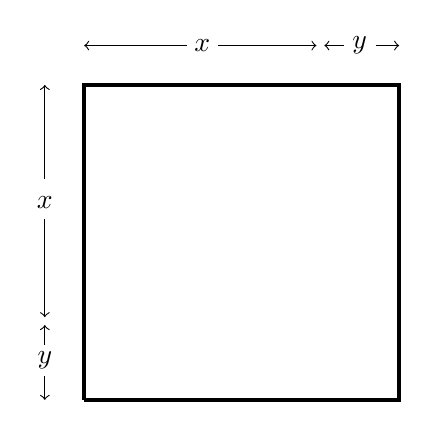
\begin{tikzpicture}
\draw[ultra thick] (0,0) -- (0,4) -- (4,4) -- (4,0) -- (0,0);
\node at (-0.5,2.5){$x$};  
\draw[<-] (-0.5,4) -- (-0.5,2.8);
\draw[->] (-0.5,2.3) -- (-0.5,1.05);
\draw[<-] (-0.5,0)--(-0.5,0.3);
\draw[->] (-0.5,0.7)--(-0.5,0.95);
\node at (-0.5,0.5){$y$};
\node at (1.5,4.5){$x$};  
\draw[<-] (0,4.5) -- (1.3,4.5);
\draw[->] (1.7,4.5) -- (2.95,4.5);
\draw[<-] (3.05,4.5)--(3.3,4.5);
\draw[->] (3.7,4.5)--(4,4.5);
\node at (3.5,4.5){$y$};
\end{tikzpicture}
\vfill
\item Next you will solve the system of equations (below) in two different ways.\\
$$xy=10 \hspace{.3in} (x+y)^2+4(x-y)=45$$
	\begin{enumerate}
	\item Solve this using the Babylonian strategy on pages 69-70. This requires using part (1) above to rewrite the second equation as a quadratic in $(x-y)$ and then solving this quadratic using a Babylonian quadratic formula. Once this is accomplished, you solve the system of the form $ x-y=a, \: xy=b$ again using the Babylonian quadratic equation.
	\vfill
	\item Solve the system using a computational tool like Wolfram Alpha or similar. What do you observe?
	\vfill
	\end{enumerate}
\end{enumerate}
\end{document}